\documentclass{article}
\usepackage{graphicx} % Required for inserting images

\title{Deep Learning Labwork 2}
\author{2440048 - Thien An NGUYEN}
\date{April 2025}

\begin{document}

\maketitle

\section{Introduction}
In this lab work, we focus on Linear Regression, where I implemented the algorithm in Python from scratch.\\
\noindent Linear Regression aims to model the relationship between inputs and outputs by fitting a straight line to the observed data. This line is represented by a linear equation. I will, of course, use Gradient Descent to update the weights. For this labwork, assume we only have 2 weights to update for the equation $y = w_0 + w_1x$\\
\noindent Linear Regression typically uses a Mean Square Error Cost Function. ($MSE = \frac{1}{N} \sum_{i=1}^{N} (y_i - (w_0 + w_1 x_i))^2$ or scaled version $MSE = \frac{1}{2}* \frac{1}{N} \sum_{i=1}^{N} (y_i - (w_0 + w_1 x_i))^2$). The gradient will be calculated for each $w_0$ and $w_1$, and then they will be updated.

\section{Implementation}
\subsection{The code}
The linear regression function:
\begin{verbatim}
def linear_regression(x, y, F, lr, iter, threshold):
    assert len(x) == len(y), "length must be the same"
    W = [0, 0]
    loss_list = []
    weights_states = []

    loss = F(x, y, W)
    print(f"Initial loss: {loss}")
    loss_list.append(loss)
    print(f"Initial weights: {W}")

    for i in range(iter):
        # calculate gradient
        J_w0 = F_w0(x, y, W)
        J_w1 = F_w1(x, y, W)

        # update the weights
        W[0] = W[0] - lr * J_w0
        W[1] = W[1] - lr * J_w1

        # calculate loss
        loss = F(x, y, W)
        loss_list.append(loss)

        # check if loss update is less than threshold
        if abs(loss_list[-1]-loss_list[-2]) < threshold:
            break

        weights_states.append(W[:])
    
    return W, loss_list, weights_states
\end{verbatim}

The cost function calculation
\begin{verbatim}
def F(x, y, W):
    J = 0
    for i in range(len(x)):
        J += (W[0] + W[1]*x[i] - y[i])**2
    J = J/(2*len(x))
    return J
\end{verbatim}

Derivative or Gradient for $w_0$ and $w_1$
\begin{verbatim}
def F_w0(x, y, W):
    J_w0 = 0
    N = len(x)
    for i in range(len(x)):
        J_w0 += (W[0] + W[1]*x[i] - y[i])
    J_w0 = J_w0/N
    return J_w0

def F_w1(x, y, W):
    J_w1 = 0 
    N = len(x)
    for i in range(len(x)):
        J_w1 += (W[0] + W[1]*x[i] - y[i])*x[i]
    J_w1 = J_w1/N
    return J_w1
\end{verbatim}

\textit{Numeric version of all of the above:}
\begin{verbatim}
def linear_regression_2(x, y, F, lr, iter, threshold):
    assert len(x) == len(y), "length must be the same"
    W = [0, 0]
    loss_list = []
    weights_states = []

    loss = F(x, y, W)
    print(f"Initial loss: {loss}")
    loss_list.append(loss)
    print(f"Initial weights: {W}")

    for i in range(iter):
        # calculate gradient
        W_0_h = [W[0] + 1e-5, W[1]]
        W_1_h = [W[0], W[1] + 1e-5]

        W_0_h_ = [W[0] - 1e-5, W[1]]
        W_1_h_ = [W[0], W[1] - 1e-5]

        J_w0 = (F(x, y, W_0_h) - F(x, y, W_0_h_)) / 2e-5
        J_w1 = (F(x, y, W_1_h) - F(x, y, W_1_h_)) / 2e-5

        # update the weights
        W[0] = W[0] - lr * J_w0
        W[1] = W[1] - lr * J_w1

        # calculate loss
        loss = F(x, y, W)
        loss_list.append(loss)

        # check if loss update is less than threshold
        if abs(loss_list[-1]-loss_list[-2]) < threshold:
            break

        weights_states.append(W[:])
        
    return W, loss_list, weights_states
\end{verbatim}

\subsection{Explanation}
My code takes the following inputs:
\begin{itemize}
    \item x: The inputs for a batch (here, since the data is small,l so it's the whole input)
    \item F: The cost function (loss function) (Here is MSE)
    \item lr: The learning rate (or the step we want to take follows the Gradient.
    \item iter: Max number of iterations
    \item threshold: The threshold at which, if the changes after each step are not too big anymore, we stop.
\end{itemize}

\noindent In my linear regression function, the weights are first initialized as [0,0], but we can modify this later and use it as an argument for the function. The loss is calculated, and then we apply the Gradient Descent. Here, I used the scaled version of MSE. For $w_0$ the analytic Gradient are pre-computed as $\frac{\partial J}{\partial w_0} = \frac{1}{N} \sum_{i=1}^{N} (w_0 + w_1 x_i - y_i)$ and $w_1$ is $\frac{\partial J}{\partial w_1} = \frac{1}{N} \sum_{i=1}^{N} (w_0 + w_1 x_i - y_i) x_i$. They will be updating my LR step towards the minimum. The numeric version is the same, but I calculated it using the central derivative formula.

\section{Experiments}
Here is the data that we are dealing with:
\begin{verbatim}
Input: [10.0, 20.0, 40.0, 60.0, 80.0]
Output: [55.0, 80.0, 100.0, 120.0, 150.0]
\end{verbatim}
Where each input has a corresponding output.

We will use the $f(x) = x^2$ function for the experiment and experiment with the learning rate of 0.0001, 0.0003, and 0.001. With max iteration is 20.

\begin{figure}[ht]
  \centering
  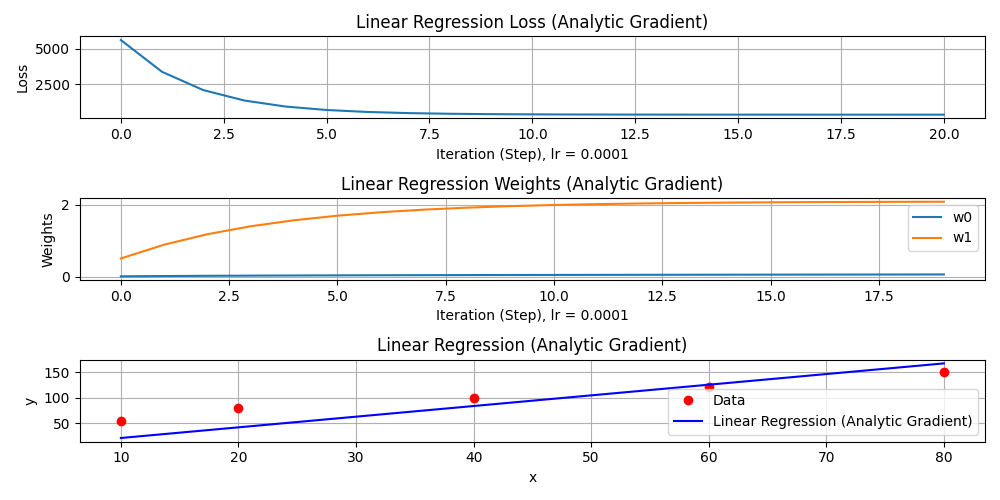
\includegraphics[width=1\textwidth]{images/lab2/linear_regression_(0.0001).png}
  \caption{Linear Regression with Learning Rate 0.0001}
  \label{fig:lr_0.0001}
\end{figure}

\begin{figure}[ht]
  \centering
  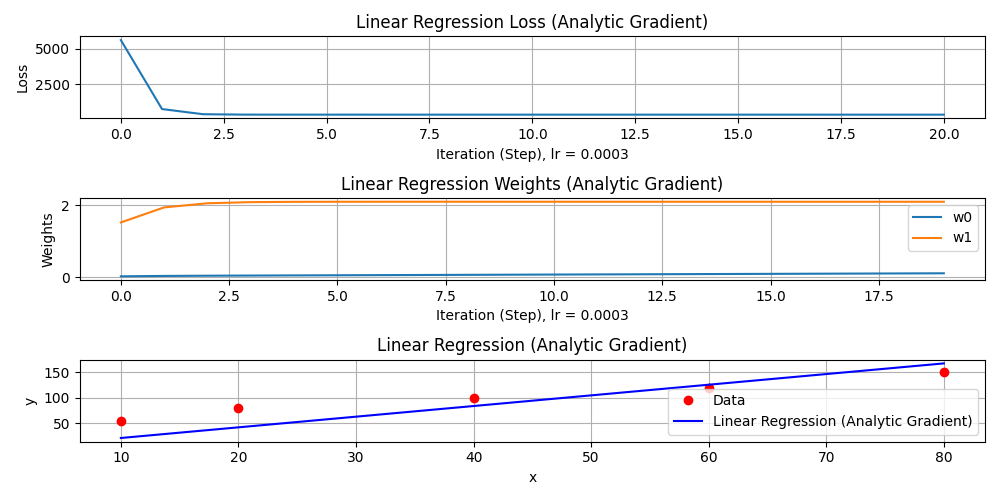
\includegraphics[width=1\textwidth]{images/lab2/linear_regression_(0.0003).png}
  \caption{Linear Regression with Learning Rate 0.0003}
  \label{fig:lr_0.0003}
\end{figure}

\begin{figure}[ht]
  \centering
  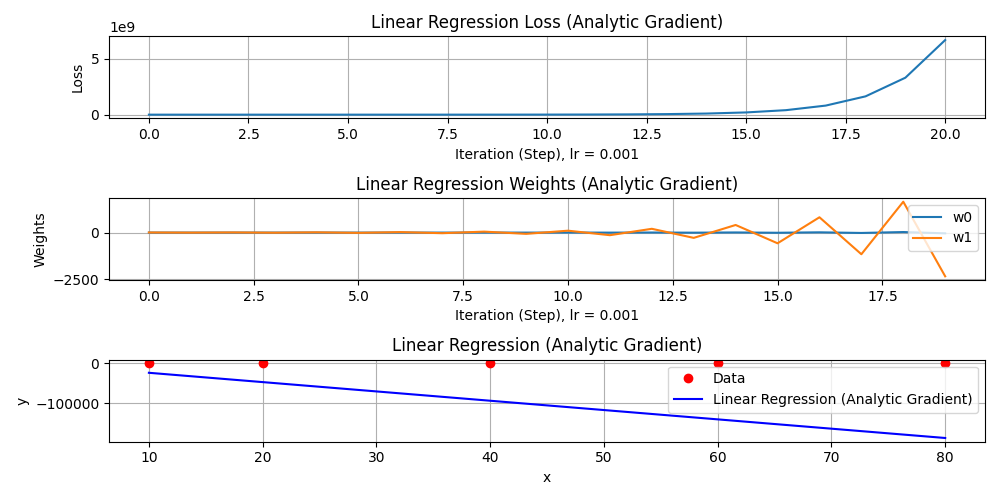
\includegraphics[width=1\textwidth]{images/lab2/linear_regression_(0.001).png}
  \caption{Linear Regression with Learning Rate 0.001}
  \label{fig:lr_0.001}
\end{figure}

\newpage
\noindent You can see that for the first two cases, the loss reduced and converged. The weights are updated accordingly. For the last case, it diverged since the learning rate was too high. These havea  similar phenomenon to Gradient Descent.\\
\noindent The line on the 2 cases fits quite well with the data, while the last case doesn't fit at all.

\end{document}
